
% RUN:
% pdflatex -output-directory=/home/salvadortorpes/Aprendizagem/Homework1/trash /home/salvadortorpes/Aprendizagem/Homework1/G22.tex

% ir a settings.json e adicionar:
% // According to the wiki, the string latex-workshop.latex.autoBuild.run has three possible values: never, onSave and onFileChange(default).
% "latex-workshop.latex.autoBuild.run": "never",

\documentclass{article}

\author{Pedro Curvo (ist1102716) \\ Salvador Torpes (ist1102474)}

\usepackage[utf8]{inputenc}
\usepackage[portuguese]{babel}
\usepackage[letterpaper,top=10mm,bottom=15mm,left=10mm,right=10mm,marginparwidth=1.75cm]{geometry}
\usepackage{multicol}
\usepackage{biblatex}
\addbibresource{Bibliografia.bib}
\usepackage{graphicx}
\usepackage{subcaption}
\usepackage{tabularx}
\usepackage{booktabs}
\usepackage{array}
\usepackage{makecell}
\usepackage{multirow}
\usepackage{amsmath}
\usepackage{makecell}
\usepackage{url}
\usepackage{csquotes}
\usepackage{caption}
\usepackage{enumitem}
\usepackage{textcomp}
\usepackage{pdflscape}
\usepackage{makeidx}
% \usepackage{tocbibind}
\providecommand{\tightlist}{\relax}
\usepackage{tocloft}
\renewcommand{\cftsecindent}{0em}
\renewcommand{\cftsubsecindent}{1em}
\renewcommand{\cftsecfont}{\bfseries}
\renewcommand{\cftsubsecfont}{\itshape}
\setlength{\cftsubsecnumwidth}{0em}

\usepackage[version=4]{mhchem}
\usepackage{hyperref} % Remove "pdftex" option here
\usepackage{float}
\usepackage{fancyhdr}
\usepackage{ragged2e}
\usepackage{xkeyval}
%\usepackage{minted}
%\usemintedstyle{manni}
\usepackage{listings}
\usepackage{amssymb}



\usepackage{xcolor}
\usepackage{tikz}
\usetikzlibrary{positioning}
\usetikzlibrary{positioning, arrows.meta}
\usepackage{adjustbox}
\usepackage{sidecap}



% \usepackage[table,xcdraw]{xcolor}

\usepackage{tikz-3dplot}
% \usepackage{pgfplots}
\usetikzlibrary{calc, 3d, arrows}
\usepackage{forest}




\usetikzlibrary{shapes.geometric, arrows}


\lstset{
    language=Python,
    basicstyle=\ttfamily,
    keywordstyle=\color{blue},
    commentstyle=\color{gray},
    stringstyle=\color{orange},
    numbers=left,
    numberstyle=\tiny,
    numbersep=5pt,
    showspaces=false,
    showstringspaces=false,
    breaklines=true,
    frame=tb,
    framexleftmargin=2em,
    xleftmargin=2em,
}


%\usepackage{fontspec}

%\setmonofont{Fira Code}

\fancyhf{}
\cfoot{\thepage}
\fancyhf{} % Clear all header and footer fields
\renewcommand{\headrulewidth}{0pt} % Remove the header rule line
\cfoot{\thepage} % Set the page number in the center of the footer

\pagestyle{fancy} % Apply the fancy page style

\setlength\columnsep{20pt}

\renewcommand{\familydefault}{\sfdefault}

\newenvironment{Figure}
  {\par\medskip\noindent\minipage{\linewidth}}
  {\endminipage\par\medskip}

\makeatletter
\newenvironment{figurehere}
{\def\@captype{figure}}
{}
\makeatother

\hypersetup{
  colorlinks,
  linkcolor=blue,
  anchorcolor=black,
  citecolor=cyan,
  filecolor=cyan,
  menucolor=cyan,
  urlcolor=cyan,
  bookmarksopen=true,
  bookmarksnumbered=true
}

\makeindex


\title{\vspace{-6mm}
\includegraphics[width=15mm,scale=3]{Homework1/images/IST_Logo.png}\\ \vspace{5mm}
Aprendizagem - HomeWork 1 \vspace{-5mm}}
\date{1º Semestre - 23/24}

\usepackage{sansmathfonts}
\usepackage[T1]{fontenc}
\usepackage[OT1]{fontenc}

\begin{document}

\renewcommand{\arraystretch}{1.5}
\setlength{\columnseprule}{0.4pt}
\tdplotsetmaincoords{70}{110} % Set the viewing angle
\newcolumntype{M}[1]{>{\centering\arraybackslash\vspace{#1}}m{0.5\linewidth}<{\vspace{#1}}}
\newcolumntype{C}[2]{>{\centering\arraybackslash\vspace{#1}\rule{0pt}{#1}\hspace{0pt}}m{#2}}
\newcolumntype{w}[1]{>{\centering\arraybackslash}m{#1}}

\renewcommand*\familydefault{\sfdefault} %% Only if the base font of the document is to be sans serif

\maketitle

\vspace{-5mm}

\hrulefill

\section{Dataset}

Considering dataset D:

\begin{table}[h!]
\centering
\begin{tabular}{|c|c|c|c|c|c|}
\hline
    D     & $y_1$ & $y_2$ & $y_3$ & $y_4$ & $y_{out}$ \\ \hline
    $x_1$ & 0.24   & 1     & 1     & 0     & A         \\ \hline
    $x_2$ & 0.06   & 2     & 0     & 0     & B         \\ \hline
    $x_3$ & 0.04   & 0     & 0     & 0     & B         \\ \hline
    $x_4$ & 0.36   & 0     & 2     & 1     & C         \\ \hline
    $x_5$ & 0.32   & 0     & 0     & 2     & C         \\ \hline
    $x_6$ & 0.68   & 2     & 2     & 1     & A         \\ \hline
    $x_7$ & 0.90   & 0     & 1     & 2     & A         \\ \hline
    $x_8$ & 0.76   & 2     & 2     & 0     & A         \\ \hline
    $x_9$ & 0.46   & 1     & 1     & 1     & B         \\ \hline
 $x_{10}$ & 0.62   & 0     & 0     & 1     & B         \\ \hline
 $x_{11}$ & 0.44   & 1     & 2     & 2     & C         \\ \hline
 $x_{12}$ & 0.52   & 0     & 2     & 0     & C         \\ \hline
\end{tabular}
\caption{Dataset D}
\label{tab:datasetD}
\end{table}

\section{Exercício 1.}

De modo a corretamente completar a árvore de decisão, é necessário calcular o Information gain (IG) da variável de output $y_{out}$ condicionada a cada uma das variáveis $y_2$, $y_3$ e $y_4$. 

\subsection{Escolha do 2º nó}

Como queremos completar o ramo $y_1>0.4$, vamos apenas considerar as ocorrencias em que $y_1>0.4$ para calcular o IG.

\paragraph{Information Gain de $y_{out}$ condicionada a $y_2$}

\[ IG(y_{out}|y_2) = H(y_{out}) - H(y_{out}|y_2) \]

\[ H(y_{out}) = \left(- \sum_{i=1}^{3} p_{out_i} (\log_2 p_{out_i})\right) = - \left( \frac{3}{7} \log_2 \left( \frac{3}{7} \right) + \frac{2}{7} \log_2 \left( \frac{2}{7} \right) + \frac{2}{7} \log_2 \left( \frac{2}{7} \right) \right) = 1.5567 \]

\[ H(y_{out}|y_2) = \sum_{i=0}^{2} p_{y_2 = i} H(y_{out}|y_2 = i) \]

Tabela dividida em 3 sub-tabelas, cada uma com os dados que verificam $y_2 = 0$, $y_2 = 1$ e $y_2 = 2$, respetivamente:

\begin{multicols}{3}
  \setlength{\columnseprule}{0pt}
  
  \begin{table}[H]
    \centering
    \begin{tabular}{|c|c|c|}
    \hline
        D     & $y_2$ & $y_{out}$ \\ \hline
        $x_7$ & 0     & A         \\ \hline
        $x_{10}$ & 0     & B         \\ \hline
        $x_{12}$ & 0     & C         \\ \hline
    \end{tabular}
    \caption{Dataset D com $y_2 = 0$}
    \label{tab:datasetDy2=0}
    \end{table}

\vspace*{\fill}
\collumnbreak

\begin{table}[H]
  \centering
  \begin{tabular}{|c|c|c|}
  \hline
      D     & $y_2$ & $y_{out}$ \\ \hline
      $x_9$ & 1     & B         \\ \hline
      $x_{11}$ & 1     & C         \\ \hline
  \end{tabular}
  \caption{Dataset D com $y_2 = 1$}
  \label{tab:datasetDy2=1}
  \end{table}

\vspace*{\fill}
\collumnbreak

\begin{table}[H]
  \centering
  \begin{tabular}{|c|c|c|}
  \hline
      D     & $y_2$ & $y_{out}$ \\ \hline
      $x_6$ & 2     & A         \\ \hline
      $x_8$ & 2     & A         \\ \hline
  \end{tabular}
  \caption{Dataset D com $y_2 = 1$}
  \label{tab:datasetDy2=1}
  \end{table}

\end{multicols}

\[ H(y_{out}|y_2 = 0) = - \left( \frac{1}{3} \log_2 \left( \frac{1}{3} \right) + \frac{1}{3} \log_2 \left( \frac{1}{3} \right) + \frac{1}{3} \log_2 \left( \frac{1}{3} \right) \right) = 1.58496 \]

\[ H(y_{out}|y_2 = 1) = - \left( \frac{1}{2} \log_2 \left( \frac{1}{2} \right) + \frac{1}{2} \log_2 \left( \frac{1}{2} \right) \right) = 1 \]

\[ H(y_{out}|y_2 = 2) = - \left( \log(1) \right) = 0 \]

Assim, podemos calcular a entropia de $y_{out}$ condicionada a $y_2$:

\[ H(y_{out}|y_2) = \frac{3}{7} H(y_{out}|y_2 = 0) + \frac{2}{7} H(y_{out}|y_2 = 1) + \frac{2}{7} H(y_{out}|y_2 = 2) = \]
\[ = \frac{3}{7} \times 1.58496 + \frac{2}{7} \times 1 + \frac{2}{7} \times 0 = 0.96498 \]

Por fim, podemos calcular o Information Gain:

\[ IG(y_{out}|y_2) = H(y_{out}) - H(y_{out}|y_2) = 1.5567 - 0.96498 = 0.59172 \]

\paragraph{Information Gain de $y_{out}$ condicionada a $y_3$}

\[ IG(y_{out}|y_3) = H(y_{out}) - H(y_{out}|y_3) \]

\[ H(y_{out}|y_3) = \sum_{i=0}^{2} p_{y_3 = i} H(y_{out}|y_3 = i) \]

Tabela dividida em 3 sub-tabelas, cada uma com os dados que verificam $y_3 = 0$, $y_3 = 1$ e $y_3 = 2$, respetivamente:

\begin{multicols}{3}
\setlength{\columnseprule}{0pt}

\vspace*{\fill}
\begin{table}[H]
\centering
\begin{tabular}{|c|c|c|}
\hline
D     & $y_3$ & $y_{out}$ \\ \hline
$x_{10}$ & 0     & B         \\ \hline
\end{tabular}
\caption{Dataset D com $y_3 = 0$}
\label{tab:datasetDy3=0}
\end{table}

\vspace*{\fill}

\collumnbreak

\begin{table}[H]
\centering
\begin{tabular}{|c|c|c|}
\hline
D     & $y_3$ & $y_{out}$ \\ \hline
$x_7$ & 1     & A         \\ \hline
$x_9$ & 1     & B         \\ \hline
\end{tabular}
\caption{Dataset D com $y_3 = 1$}
\label{tab:datasetDy3=1}
\end{table}


\vspace*{\fill}
\collumnbreak

\begin{table}[H]
\centering
\begin{tabular}{|c|c|c|}
\hline
D     & $y_3$ & $y_{out}$ \\ \hline
$x_6$ & 2     & A         \\ \hline
$x_8$ & 2     & A         \\ \hline
$x_{11}$ & 2     & C         \\ \hline
$x_{12}$ & 2     & C         \\ \hline
\end{tabular}
\caption{Dataset D com $y_3 = 2$}
\label{tab:datasetDy3=2}
\end{table}
\end{multicols}

\[ H(y_{out}|y_3 = 0) = - \left( \log(1) \right) = 0 \]

\[ H(y_{out}|y_3 = 1) = - \left( \frac{1}{2} \log_2 \left( \frac{1}{2} \right) + \frac{1}{2} \log_2 \left( \frac{1}{2} \right) \right) = 1 \]

\[ H(y_{out}|y_3 = 2) = - \left( \frac{2}{4} \log_2 \left( \frac{2}{4} \right) + \frac{2}{4} \log_2 \left( \frac{2}{4} \right) \right) = 1 \]

Assim, podemos calcular a entropia de $y_{out}$ condicionada a $y_3$:

\[ H(y_{out}|y_3) = \frac{1}{7} H(y_{out}|y_3 = 0) + \frac{2}{7} H(y_{out}|y_3 = 1) + \frac{4}{7} H(y_{out}|y_3 = 2) = \]

\[ = \frac{1}{7} \times 0 + \frac{2}{7} \times 1 + \frac{4}{7} \times 1 = 0.85714 \]

Por fim, podemos calcular o Information Gain:

\[ IG(y_{out}|y_3) = H(y_{out}) - H(y_{out}|y_3) = 1.5567 - 0.85714 = 0.69956 \]

\paragraph{Information Gain de $y_{out}$ condicionada a $y_4$}

\[ IG(y_{out}|y_4) = H(y_{out}) - H(y_{out}|y_4) \]

\[ H(y_{out}|y_4) = \sum_{i=0}^{2} p_{y_4 = i} H(y_{out}|y_4 = i) \]

Tabela dividida em 3 sub-tabelas, cada uma com os dados que verificam $y_4 = 0$, $y_4 = 1$ e $y_4 = 2$, respetivamente:

\begin{multicols}{3}
\setlength{\columnseprule}{0pt}

\vspace*{\fill}
\begin{table}[H]
\centering
\begin{tabular}{|c|c|c|}
\hline  
D     & $y_4$ & $y_{out}$ \\ \hline
$x_8$ & 0     & A         \\ \hline
$x_{12}$ & 0     & C         \\ \hline
\end{tabular}
\caption{Dataset D com $y_4 = 0$}
\label{tab:datasetDy4=0}
\end{table}

\vspace*{\fill}
\collumnbreak

\begin{table}[H]
\centering
\begin{tabular}{|c|c|c|}
\hline
D     & $y_4$ & $y_{out}$ \\ \hline
$x_6$ & 1     & A         \\ \hline
$x_9$ & 1     & B         \\ \hline
$x_{10}$ & 1     & B         \\ \hline
\end{tabular}
\caption{Dataset D com $y_4 = 1$}
\label{tab:datasetDy4=1}
\end{table}

\vspace*{\fill}
\collumnbreak

\begin{table}[H]
\centering
\begin{tabular}{|c|c|c|}
\hline
D     & $y_4$ & $y_{out}$ \\ \hline
$x_7$ & 2     & A         \\ \hline
$x_{11}$ & 2     & C         \\ \hline
\end{tabular}
\caption{Dataset D com $y_4 = 2$}
\label{tab:datasetDy4=2}
\end{table}

\end{multicols}

\[ H(y_{out}|y_4 = 0) = - \left( \frac{1}{2} \log_2 \left( \frac{1}{2} \right) + \frac{1}{2} \log_2 \left( \frac{1}{2} \right) \right) = 1 \]

\[ H(y_{out}|y_4 = 1) = - \left( \frac{2}{3} \log_2 \left( \frac{2}{3} \right) + \frac{1}{3} \log_2 \left( \frac{1}{3} \right) \right) = 0.918295 \]

\[ H(y_{out}|y_4 = 2) = - \left( \frac{1}{2} \log_2 \left( \frac{1}{2} \right) + \frac{1}{2} \log_2 \left( \frac{1}{2} \right) \right) = 1 \]

Assim, podemos calcular a entropia de $y_{out}$ condicionada a $y_4$:

\[ H(y_{out}|y_4) = \frac{2}{7} H(y_{out}|y_4 = 0) + \frac{3}{7} H(y_{out}|y_4 = 1) + \frac{2}{7} H(y_{out}|y_4 = 2) = \]

\[ = \frac{2}{7} \times 1 + \frac{3}{7} \times 0.918295 + \frac{2}{7} \times 1 = 0.96498 \]

Por fim, podemos calcular o Information Gain:

\[ IG(y_{out}|y_4) = H(y_{out}) - H(y_{out}|y_4) = 1.5567 - 0.96498 = 0.59172 \]

\paragraph{Comparação dos IG}

Podemos confirmar, pelos cálculos acima, que:

\[ IG(y_{out}|y_2) = IG(y_{out}|y_4) < IG(y_{out}|y_3) \]

Assim, a variável $y_3$ é a que tem maior IG, pelo que é a variável que escolhemos para o 2º nó da árvore de decisão no ramo $y_1>0.4$.
Este nó vai ter três ramos, um para cada valor possível de $y_3$: a ocorrência $y_3=0$ tem apenas uma ocorrência e a ocorrência $y_3=1$ tem apenas duas ocorrências, pelo que estes dois nós não são expandidos.
Por outro lado, $y_3=2$ tem 4 ocorrências, pelo que é o único nó que é expandido. Falta averiguar qual a variável que vai ser usada para expandir este nó.

\subsection{Escolha do 3º nó}

Queremos agora completar o ramo que verifica $y_1 > 0.4$ e $y_3 = 2$. Para isso, vamos calcular o IG de $y_{out}$ para $y_2$ e $y_4$ considerando apenas as ocorrências que verificam $y_1 > 0.4$ e $y_3 = 2$:

\paragraph{Information Gain de $y_{out}$ condicionada a $y_2$}

\[ IG(y_{out}|y_2) = H(y_{out}) - H(y_{out}|y_2) \]

\[ H(y_{out}) = \left(- \sum_{i=1}^{3} p_{out_i} (\log_2 p_{out_i})\right) = - \left( \frac{2}{4} \log_2 \left( \frac{2}{4} \right) + \frac{2}{4} \log_2 \left( \frac{2}{4} \right) \right) = 1 \]

\[ H(y_{out}|y_2) = \sum_{i=0}^{2} p_{y_2 = i} H(y_{out}|y_2 = i) \]

As entropias condicionadas de $y_{out}$ para cada valor de $y_2$ são:

\[ H(y_{out}|y_2 = 0) = - \left( \log_2(1) \right) = 0 \]

\[ H(y_{out}|y_2 = 1) = - \left( \log_2(1) \right) = 0 \]

\[ H(y_{out}|y_2 = 2) = - \left( \log_2(1) \right) = 0 \]

Assim, podemos calcular a entropia de $y_{out}$ condicionada a $y_2$:

\[ H(y_{out}|y_2) = \frac{1}{4} H(y_{out}|y_2 = 0) + \frac{1}{4} H(y_{out}|y_2 = 1) + \frac{2}{4} H(y_{out}|y_2 = 2) = \]

\[ = \frac{1}{4} \times 0 + \frac{1}{4} \times 0 + \frac{2}{4} \times 0 = 0 \]

Por fim, podemos calcular o Information Gain:

\[ IG(y_{out}|y_2) = H(y_{out}) - H(y_{out}|y_2) = 1 - 0 = 1 \]

\paragraph{Information Gain de $y_{out}$ condicionada a $y_4$}

\[ IG(y_{out}|y_4) = H(y_{out}) - H(y_{out}|y_4) \]

\[ H(y_{out}|y_4) = \sum_{i=0}^{2} p_{y_4 = i} H(y_{out}|y_4 = i) \]

As entropias condicionadas de $y_{out}$ para cada valor de $y_4$ são:

\[ H(y_{out}|y_4 = 0) = - \left( \frac{1}{2} \log_2 \left( \frac{1}{2} \right) + \frac{1}{2} \log_2 \left( \frac{1}{2} \right) \right) = 1 \]

\[ H(y_{out}|y_4 = 1) = - \left( \log_2(1) \right) = 0 \]

\[ H(y_{out}|y_4 = 2) = - \left( \log_2(1) \right) = 0 \]

Assim, podemos calcular a entropia de $y_{out}$ condicionada a $y_4$:

\[ H(y_{out}|y_4) = \frac{2}{4} H(y_{out}|y_4 = 0) + \frac{1}{4} H(y_{out}|y_4 = 1) + \frac{1}{4} H(y_{out}|y_4 = 2) = \]

\[ = \frac{2}{4} \times 1 + \frac{1}{4} \times 0 + \frac{1}{4} \times 0 = 0.5 \]

Por fim, podemos calcular o Information Gain:

\[ IG(y_{out}|y_4) = H(y_{out}) - H(y_{out}|y_4) = 1 - 0.5 = 0.5 \]

\paragraph{Comparação dos IG}

Podemos confirmar, pelos cálculos acima, que:

\[ IG(y_{out}|y_2) > IG(y_{out}|y_4) \]

Assim, a variável $y_2$ é a que tem maior IG, pelo que é a variável que escolhemos para o 3º nó da árvore de decisão no ramo $y_1>0.4$ e $y_3 = 2$.
Todos os nós desta árvore têm menos que 4 ocorrências, pelo que nehum deles é expandido e termina a árvore de decisão.


\subsection{Construção da árvore de decisão}

Para completar a árvore, resta preencher os nós terminais com os valores de $y_{out}$ que são mais prováveis em cada ramo. Em caso de empate, escolhemos por ordem alfabética.
A árvore de decisão final é:

\begin{center}
  \begin{forest}
  for tree={
    edge={->},
    parent anchor=south,
    child anchor=north,
    align=center,
    base=top,
    draw,
    font=\sffamily,
    s sep=9mm, % Vertical separation between siblings
    l sep=10mm, % Horizontal separation between parent and child nodes
  }
  [y_1, circle
    [$y_2$, edge label={node[midway,above]{ $ \leq 0.4$}}, circle
      [C, diamond, label = {$ = 0$}]
      [A, diamond, label = {$ = 1$}]
      [B, diamond, label = {$ = 2$}]
    ]
    [$y_3$, edge label={node[midway,above]{ $ > 0.4$}}, circle
      [B, diamond, label = {$ = 0$}]
      [A, diamond, label = {$ = 1$}]
      [$y_2$, circle, label = {$ = 2$}
        [C, diamond, label = {$ = 0$}]
        [C, diamond, label = {$ = 1$}]
        [A, diamond, label = {$ = 2$}]
      ]
    ]
  ]
  \end{forest}
  
\end{center}

\section{Exercício 2.}

Com o objetivo de desenhar a matriz de confusão da árvore de decisão construída acima, começamos por calcular os valores previstos para o output, $\hat{y}_{out}$, para cada uma das ocorrências do dataset D:

\begin{table}[h!]
\centering
\begin{tabular}{|c|c|c|c|c|c|c|}
\hline
    D     & $y_1$ & $y_2$ & $y_3$ & $y_4$ & $\hat{y}_{out}$ & $y_{out}$ \\ \hline
    $x_1$ & 0.24   & 1     & 1     & 0     & A         & A         \\ \hline
    $x_2$ & 0.06   & 2     & 0     & 0     & B         & B         \\ \hline
    $x_3$ & 0.04   & 0     & 0     & 0     & C         & B         \\ \hline
    $x_4$ & 0.36   & 0     & 2     & 1     & C         & C         \\ \hline
    $x_5$ & 0.32   & 0     & 0     & 2     & C         & C         \\ \hline
    $x_6$ & 0.68   & 2     & 2     & 1     & A         & A         \\ \hline
    $x_7$ & 0.90   & 0     & 1     & 2     & A         & A         \\ \hline
    $x_8$ & 0.76   & 2     & 2     & 0     & A         & A         \\ \hline
    $x_9$ & 0.46   & 1     & 1     & 1     & A         & B         \\ \hline
  $x_{10}$ & 0.62   & 0     & 0     & 1     & B         & B         \\ \hline
  $x_{11}$ & 0.44   & 1     & 2     & 2     & C         & C         \\ \hline
  $x_{12}$ & 0.52   & 0     & 2     & 0     & C         & C         \\ \hline
\end{tabular}
\caption{Dataset D com $\hat{y}_{out}$}
\label{tab:datasetD_comprev}
\end{table}

Assim, desenhamos a \textbf{matriz de confusão}:

\begin{table}[h!]
\centering
\begin{tabular}{|c|cccc|}
\hline
  & \multicolumn{4}{c|}{Valores reais}                                           \\ \hline
\multirow{4}{*}{\rotatebox[origin=c]{90}{Valores Previstos}} & \multicolumn{1}{c|}{} & \multicolumn{1}{c|}{A} & \multicolumn{1}{c|}{B} & C \\ \cline{2-5} 
  & \multicolumn{1}{c|}{A} & \multicolumn{1}{c|}{4} & \multicolumn{1}{c|}{1} & 0 \\ \cline{2-5} 
  & \multicolumn{1}{c|}{B} & \multicolumn{1}{c|}{0} & \multicolumn{1}{c|}{2} & 0 \\ \cline{2-5} 
  & \multicolumn{1}{c|}{C} & \multicolumn{1}{c|}{0} & \multicolumn{1}{c|}{1} & 4 \\ \hline
\end{tabular}
\end{table}

\begin{center}
  \begin{figure}[h!]
    \centering
    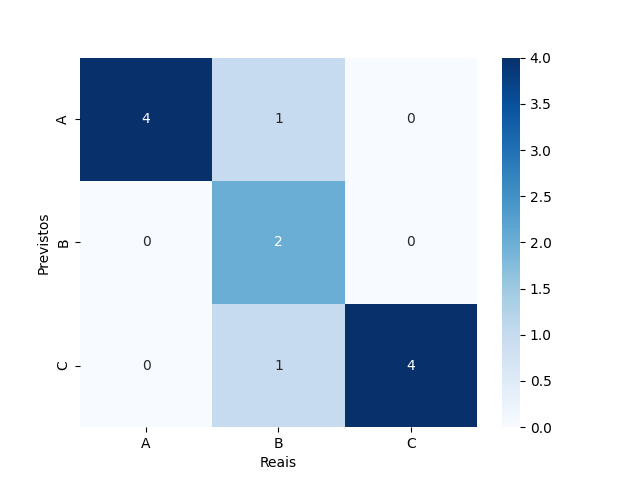
\includegraphics[width=0.5\textwidth]{Homework1/images/confusion_matrix.png}
    \caption{Matriz de confusão}
    \label{fig:confusion_matrix}
  \end{figure}
\end{center}




\end{document}